\documentclass[a4paper,11pt]{article}
\usepackage[left=2.5cm, right=2.5cm, top=2cm, bottom=1.5cm]{geometry}
\usepackage{graphicx}
\usepackage{amssymb}
\usepackage{amsmath}
\usepackage{listings}
\usepackage[utf8]{inputenc}
\usepackage{color} %red, green, blue, yellow, cyan, magenta, black, white
\definecolor{mygreen}{RGB}{28,172,0} % color values Red, Green, Blue
\definecolor{mylilas}{RGB}{170,55,241}

\begin{document}
\title{\LARGE{\textbf{ECEN 220 Lab 4}}}
\author{Niels Clayton \\300437590}
\date{September 26, 2019}
\maketitle
\hrule

\lstset{language=Matlab,%
    %basicstyle=\color{red},
    breaklines=true,%
    morekeywords={matlab2tikz},
    keywordstyle=\color{blue},%
    morekeywords=[2]{1}, keywordstyle=[2]{\color{black}},
    identifierstyle=\color{black},%
    stringstyle=\color{mylilas},
    commentstyle=\color{mygreen},%
    showstringspaces=false,%without this there will be a symbol in the places where there is a space
    numbers=left,%
    numberstyle={\tiny \color{black}},% size of the numbers
    numbersep=9pt, % this defines how far the numbers are from the text
    emph=[1]{for,end,break},emphstyle=[1]\color{red}, %some words to emphasise
    %emph=[2]{word1,word2}, emphstyle=[2]{style},    
}


\section{Computing the DTFT in MATLAB}
Below is the DTFT function written to compute figures 1 and 2:\\\\

\lstinputlisting{dtft.m}

\begin{figure}[h]
 \begin{center}
  \fbox{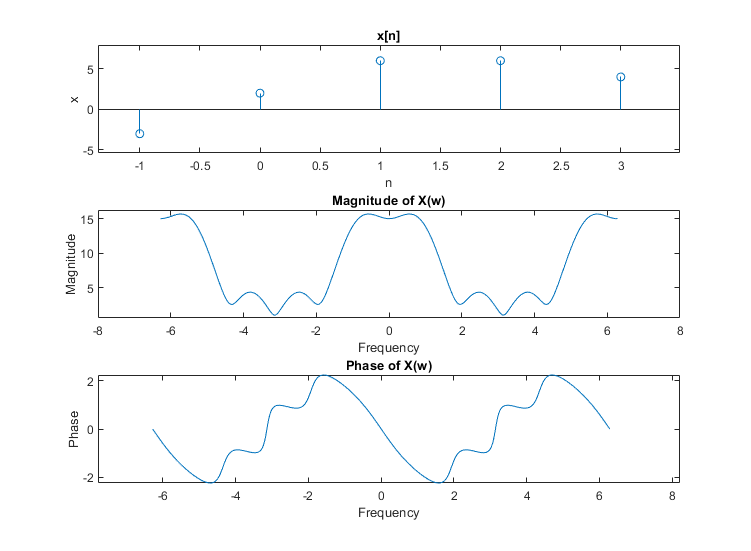
\includegraphics[width = \textwidth]{1.png}}
  \caption{DTFT of signal $x[n]$}
 \end{center}
\end{figure}

\pagebreak
\begin{figure}[h]
 \begin{center}
  \fbox{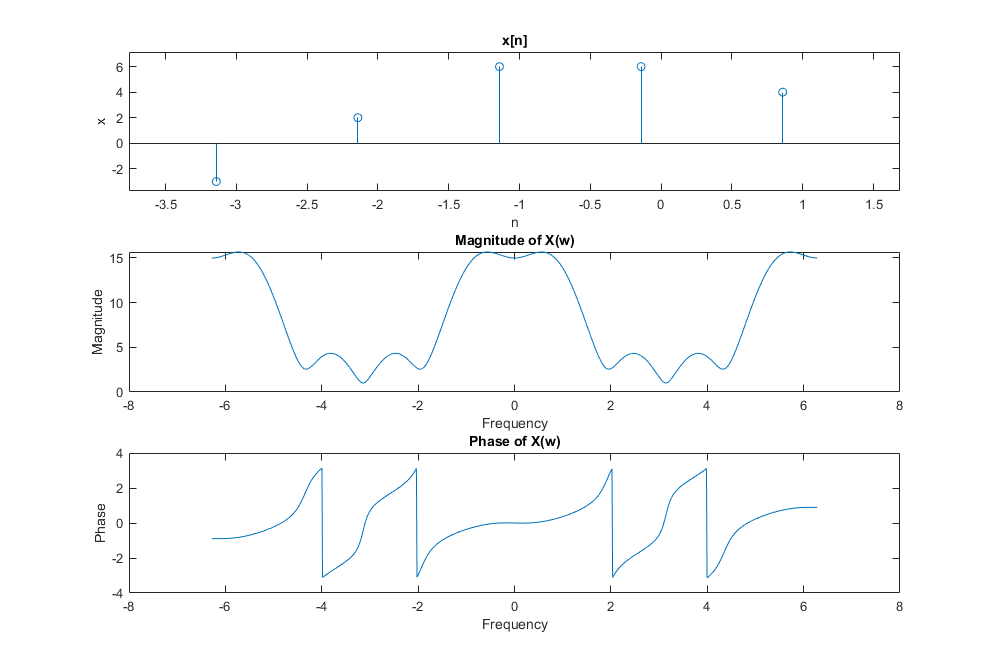
\includegraphics[width = \textwidth]{1_shift.png}}
  \caption{DTFT of signal $x[n + \pi]$}
 \end{center}
\end{figure}


By changing the position of $n=0$ we are shifting in the time domain, which will lead to a change in the phase in the frequency domain. This can be seen in the differences between figured 1 which is the DTFT of $x[n]$ and figure 2 which is the DTFT of $x[n+\pi]$.

\pagebreak
\section{Inverse DTFT in MATLAB}

Below is the inverse DTFT function written to compute figures 1 and 2:\\\\

\lstinputlisting{invdtft.m}

\begin{figure}[h]
 \begin{center}
  \fbox{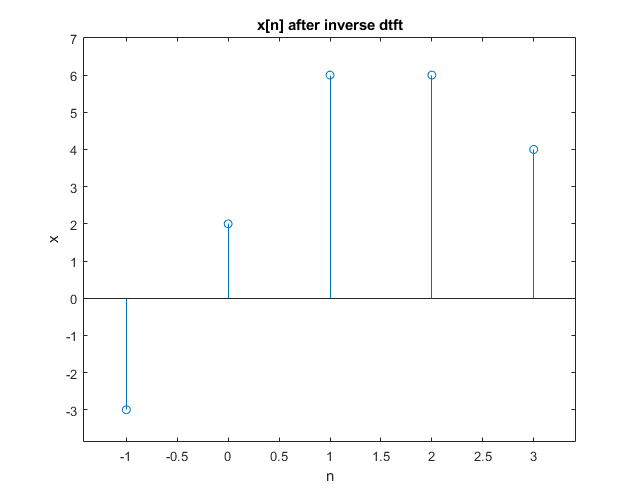
\includegraphics[width = 0.7\textwidth]{2.png}}
  \caption{Inverse DTFT of $X(e^{j\omega})$}
 \end{center}
\end{figure}

When taking the inverse discrete time Fourier transform of $X(e^{j\omega})$, it can be seen in figure 3 that the output $x[n]$ is exactly the same as the original signal. Within MATLAB however, every point of $x[n]$ is now considered to be a complex number with an imaginary component of $0i$. This is due to the nature of MATLAB functions, where if there are computations with complex numbers then the output will always be complex, even it it is solely real.

\pagebreak
\section{Filters}
\begin{figure}[h]
 \begin{center}
  \fbox{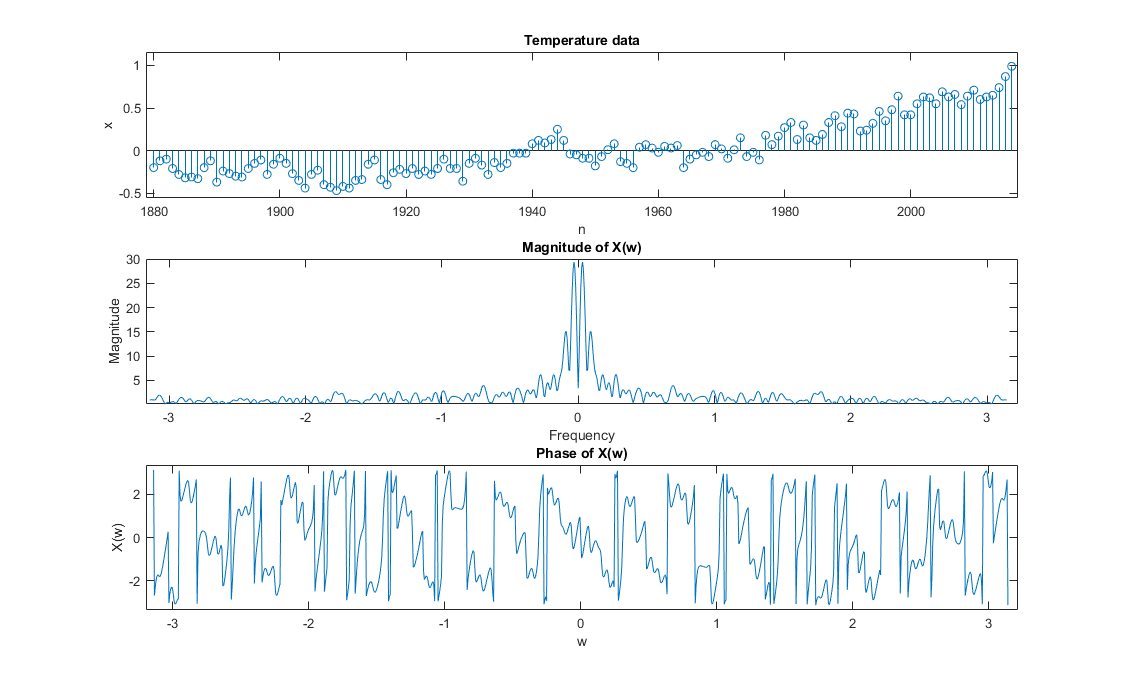
\includegraphics[width = 0.9\textwidth]{3_1.png}}
  \caption{DTFT of temperature data}
  \vspace{-20pt}
 \end{center}
\end{figure}


\begin{figure}[h]
 \begin{center}
 \vspace{-10pt}
  \fbox{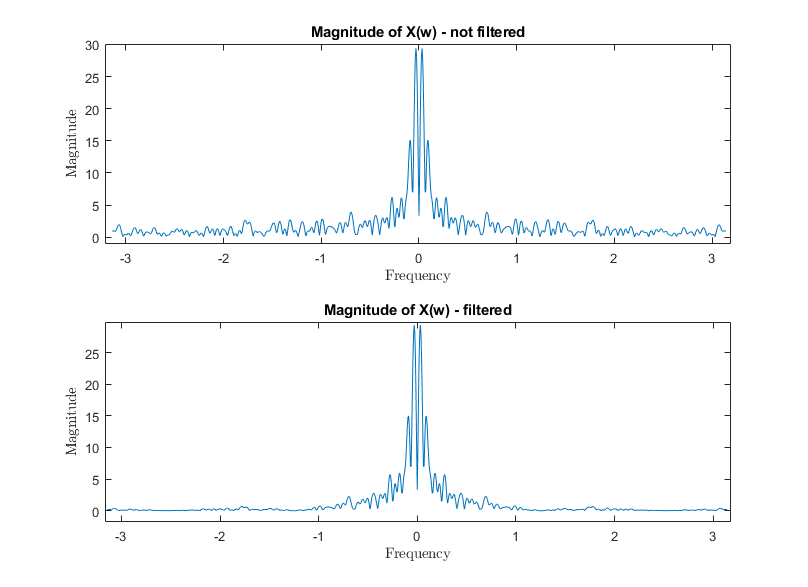
\includegraphics[width = .8\textwidth]{3_2_5.png}}
  \caption{Comparison of un-filtered and filtered data}
  \vspace{-60pt}
 \end{center}
\end{figure}

\pagebreak

\begin{figure}[h]
 \begin{center}
  \fbox{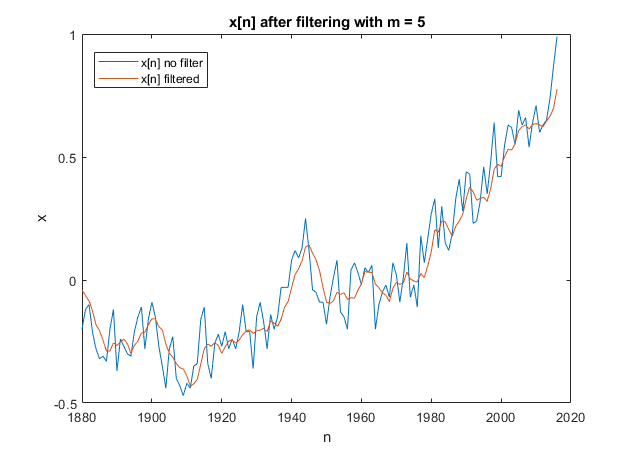
\includegraphics[width = 0.8\textwidth]{filter_5.png}}
  \caption{DTFT of temperature data}
  \vspace{-20pt}
 \end{center}
\end{figure}


\begin{figure}[h]
 \begin{center}
 \vspace{-10pt}
  \fbox{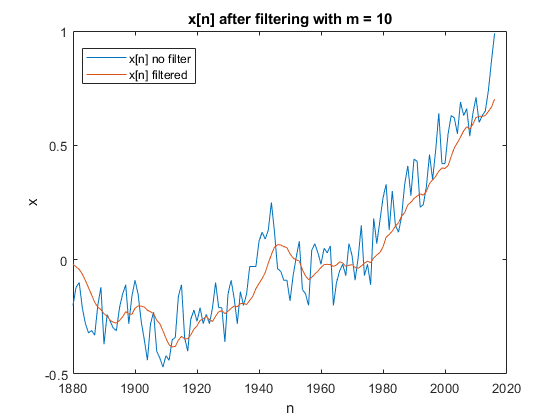
\includegraphics[width = .8\textwidth]{filter_10.png}}
  \caption{Comparison of un-filtered and filtered data}
  \vspace{-30pt}
 \end{center}
\end{figure}
\hfill\\
\hfill\\
It can be seen that as the value of $m$ increases, the amount of averaging done to the function increases as well.

\pagebreak
\section{Extra - High-pass \& Low-pass filters}

\begin{figure}[h]
 \begin{center}
  \fbox{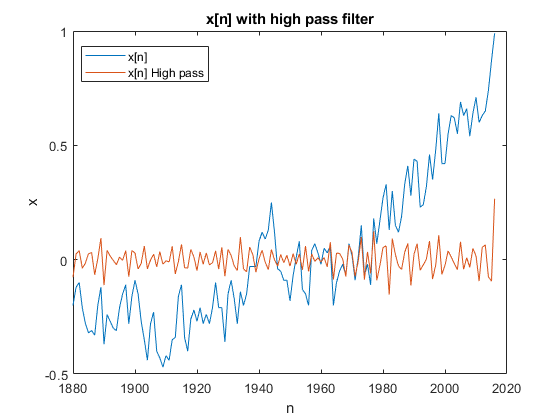
\includegraphics[width = 0.7\textwidth]{high.png}}
  \caption{DTFT of temperature data}
  \vspace{-20pt}
 \end{center}
\end{figure}


\begin{figure}[h]
 \begin{center}
 \vspace{-10pt}
  \fbox{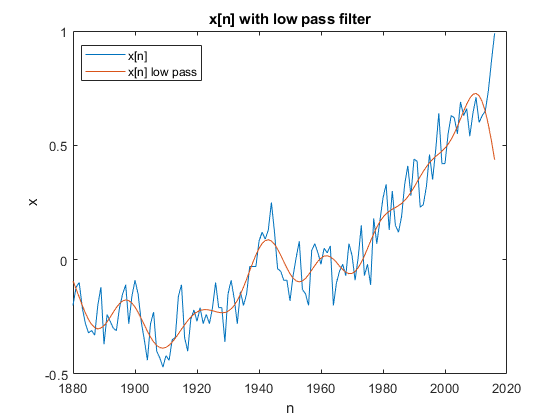
\includegraphics[width = .7\textwidth]{low.png}}
  \caption{Comparison of un-filtered and filtered data}
  \vspace{-30pt}
 \end{center}
\end{figure}
\hfill\\
\hfill\\

When passing $X(e^{j\omega})$ through a high pass filter, it can be seen in figure 8 that only the high frequency oscillations are left over, and the low frequency oscillations are removed. this means that the low frequency oscillations are responsible for the overall upwards trend in the data. When passing $X(e^{j\omega})$ through a low pass filter, this upwards trend in temperature can more distinctly be recognised.

\pagebreak
\section*{Matlab Code}

\lstinputlisting{lab_4.m}

\end{document}
